\chapter{Divergent series}
\index{divergent series}

\label{2011-m-ch-ds}
In this final chapter we will consider {\em divergent series}, which sometimes occur
in physical situations;
for instance in celestial mechanics or in quantum field theory
\cite[-30mm]{Boyd99thedevil,PhysRev.85.631,PhysRevD.57.1144,PhysRevD.62.076001}.
According to Abel\cite{Hardy:1949,Boyd99thedevil} they
appear to be the ``invention of the devil,'' and one may wonder with him~\cite{rousseau-2004} why {\em ``for the most part,
it is true that the results are correct, which is very strange.''}
There appears to be another, complementary, view on diverging series,
a view that has been expressed by Berry as follows\cite{berry-92}:
{\em ``$\ldots$ an asymptotic series $\ldots$ is a compact encoding of a function,
and its divergence should be regarded not as a deficiency but as a source of information about the function.''
}

\section{Convergence and divergence}
Let us first define {\em convergence} in the context of series.
\index{convergence}
A series
\begin{equation}
\sum_{j=0}^\infty a_j =a_0+a_1+a_2+\cdots
\end{equation}
is said to converge to the {\em sum}
$s$, if the {\em partial sum}
\begin{equation}
s_n=  \sum_{j=0}^n a_j =a_0+a_1+a_2+\cdots + a_n
\end{equation}
tends to a finite limit $s$ when $n\rightarrow \infty$;
otherwise it is said to be divergent.
\index{divergence}

% https://www.coursera.org/learn/advanced-calculus/lecture/koIrf/does-the-series-1-1-2-1-3-converge-or-diverge
A widely known diverging series is the
{\em harmonic series}
\index{harmonic series}
\begin{equation}
s=  \sum_{j=1}^\infty \frac{1}{j} = 1+\frac{1}{2}+\frac{1}{3}+\frac{1}{4}+\cdots .
\end{equation}
A medieval proof by Oresme (cf. p.~92 of Ref.~\cite[10mm]{Edwards-1979})
uses approximations: Oresme points out that increasing numbers of summands in the series can be rearranged to yield numbers bigger than, say, $\frac{1}{2}$;
more explicitly,
$\frac{1}{3}+\frac{1}{4}> \frac{1}{4}+\frac{1}{4}  =\frac{1}{2}$,
$\frac{1}{5}+ \cdots +\frac{1}{8} > 4 \frac{1}{8}  =\frac{1}{2}$,
$\frac{1}{9}+ \cdots +\frac{1}{16} > 8 \frac{1}{16}  =\frac{1}{2}$,
and so on, such that the entire series must grow larger as $\frac{n}{2}$.
As $n$ approaches infinity, the series is unbounded and thus diverges.


For the sake of further considerations let us introduce a generalization of the harmonic series:
the Riemann zeta function (sometimes also referred to as the Euler-Riemann zeta function)
\index{zeta function}
\index{Riemann zeta function}
\index{Euler-Riemann zeta function}
defined for $\Re t > 1$ by
\begin{equation}
\zeta (t) \stackrel{{\rm def}}{=}
\sum_{n=1}^\infty \frac{1}{n^t}
=
\prod_{p\;{\rm prime}} \left(\sum_{n=1}^\infty p^{-nt}\right)
=
\prod_{p\;{\rm prime}} \frac{1}{1-\frac{1}{p^t}}
\label{2016-m-ds-zeta}
\end{equation}
can be  continued analytically to all complex values $t\neq 1$, so that, for $t=-1$,
$\zeta (-1) = \sum_{n=1}^\infty n = 1+2+3+4+5 + \cdots $.
It will be re-defined later in Eq.~(\ref{2016-m-ch-ds-natnumser}).


One of the most prominent divergent series is Grandi's series, sometimes also referred to as
\index{Grandi's series}
\index{Leibniz's series}
Leibniz series~\cite{leibnitz-1860,moore-1938,Hardy:1949,everest-2003}
\begin{equation}
s = \sum_{j=0}^\infty (-1)^j=1-1+1-1+1-\cdots ,
\label{2009-fiftyfifty-1s}
\end{equation}
whose summands may be -- inconsistently
-- ``rearranged,''
yielding
\begin{equation*}
\begin{split}
\textrm{ either }
1-1+1-1+1-1+\cdots = (1-1)+(1-1)+(1-1)-\cdots =0\\
\textrm{ or }
1-1+1-1+1-1+\cdots = 1+(-1+1)+ (-1+1) +\cdots =1.
\end{split}
\end{equation*}
One could tentatively associate the arithmetical average $1/2$ to represent ``the sum of Grandi's series.''

Another tentative approach  would be to first regularize this nonconverging expression by introducing a ``small entity''
$\varepsilon$ with $0 < \varepsilon <1$, such that $\vert \varepsilon - 1 \vert  <1$, which allows to formally sum up the geometric series
\begin{equation*}
s_\varepsilon \stackrel{\text{def}}{=} \sum_{j=0}^\infty (\varepsilon -1)^j=\frac{1}{1-(\varepsilon -1)}   =\frac{1}{2- \varepsilon  };
\end{equation*}
and then take the limit $s \stackrel{\text{def}}{=}  \lim_{\varepsilon \rightarrow 0^+} s_\varepsilon
= \lim_{\varepsilon \rightarrow 0^+}  1/(2- \varepsilon  ) =   1/2$.

Indeed, by {\em Riemann's rearrangement theorem},
\index{Riemann rearrangement theorem}
convergent series  which do not absolutely converge
(i.e., $\sum_{j=0}^n a_j$ converges but $\sum_{j=0}^n \left| a_j \right|$ diverges)
can converge to any arbitrary (even infinite) value
by permuting (rearranging) the (ratio of) positive and negative terms
(the series of which must both be divergent).



\section{Abel summation}
\index{Abel sum}

Grandi's series is a particular ``disallowed'' case $q=-1$ of a {\em geometric series}
\index{geometric series}
\begin{equation}
s(q) = \sum_{j=0}^\infty q^j=1+q+q^2+q^3+ \cdots  =1+q s
\label{2009-fiftyfifty-1sgs}
\end{equation}
which, since $s(q)=1+q s(q)$, for $\vert q\vert <1$ converges  to
\begin{equation}
s(q)= \sum_{j=0}^\infty q^j= \frac{1}{1-q}.
\label{2012-fiftyfifty-1sgscont}
\end{equation}
One way to sum Grandi's series is by ``continuing''
Eq. (\ref{2012-fiftyfifty-1sgscont})
for arbitrary $q\neq 1$, thereby defining the
{\em Abel sum}
\index{Abel sum}
\begin{equation}
s=\sum_{j=0}^\infty(-1)^j  = 1-1+1-1+1-1+\cdots \stackrel{{\rm A}}{=} \frac{1}{1-(-1)} = \frac{1}{2}.
\label{2012-fiftyfifty-1sgscont1}
\end{equation}


Another divergent series,
which can be obtained by formally  expanding  the square of the Abel sum of
Grandi's series
$
s^2 \stackrel{{\rm A}}{=} [1-(-x)]^{-2} = (1+x)^{-2}
$ for  $x=1$
into the Taylor series\cite{Kline-83}
around $t=0$, and using   $(-1)^{j-1}=(-1)^{j-1}(-1)^{2}=(-1)^{j+1}$:
\begin{equation}
\begin{split}
s^2   \stackrel{{\rm A}}{=} (1+x)^{-2}  \Big|_{x =1}=
\sum_{k=0}^\infty \frac{1}{k!}\left.\left[\frac{d^k}{d{t}^k}  (1+t)^{-2}\right]   (x-t)^k\right|_{t=0, x=1}
\\
=
\sum_{k=0}^\infty (-1)^k (k+1) =
\sum_{k=0}^\infty (-1)^{k+1} k =
1-2+3-4+5-\cdots
.
\label{2009-fiftyfifty-1s1}
\end{split}
\end{equation}
On the other hand, squaring the Grandi's series yields the Abel sum
\index{Grandi's series}
\begin{equation}
s^2 =
\left(\sum_{j=0}^\infty (-1)^j\right)
\left(\sum_{k=0}^\infty (-1)^k\right)
\stackrel{{\rm A}}{=} \left(\frac{1}{2}\right)^2=\frac{1}{4},
\end{equation}
so that, one could infer the Abel sum
\begin{equation}
s^2 =
1-2+3-4+5-\cdots  \stackrel{{\rm A}}{=} \frac{1}{4}.
\end{equation}


Once this identification is established, all of Abel's hell breaks loose:
One could, for instance, ``compute the finite sum of all natural numbers''
(a sum even mentioned on page~22 in a book on String Theory~\cite{polchinski_1998}) {\it via}
\begin{equation}
S  =
\sum_{j=0}^\infty j = 1+2+3+4+5 + \cdots \stackrel{{\rm A}}{=} - \frac{1}{12}
\label{2016-m-ch-ds-natnumser}
\end{equation}
by sorting out
\begin{equation}
\begin{split}
S - \frac{1}{4}\stackrel{{\rm A}}{=}
S-s^2  = 1+2+3+4+5 + \cdots -
(1-2+3-4+5-\cdots )   \\
= 4 + 8+ 12 +  \cdots = 4 S
,
\label{2016-m-ch-ds-natnumser2}
\end{split}
\end{equation}
so that  $3 S
\stackrel{{\rm A}}{=}  - \frac{1}{4}$,
and, finally, $S
\stackrel{{\rm A}}{=}  - \frac{1}{12}$.

Note that the sequence of the partial sums $s^2_n=\sum_{j=0}^n (-1)^{j+1} j $
of $s^2$, as expanded in (\ref{2009-fiftyfifty-1s1}),
yield every integer once; that is,
$s^2_0 =0$,
$s^2_1 =0+1=1$,
$s^2_2 =0+1-2=-1$,
$s^2_3 =0+1-2+3=2$,
$s^2_4 =0+1-2+3-4=-2$,
$\ldots$,
$s^2_n =-\frac{n}{2}$ for even $n$,
and
$s^2_n =-\frac{n+1}{2}$ for odd $n$.
It thus establishes a strict one-to-one mapping
$s^2: {\Bbb N} \mapsto {\Bbb Z}$
of the natural numbers onto the integers.







\section{Borel's resummation method -- ``The Master forbids it''}
\index{Borel sum}

In what follows we shall review\cite[-50mm]{rousseau-2004}
a resummation method
\sidenote[][-30mm]{For more resummation techniques, please see Chapter 16 of
\cite{Kleinert-Schulte}
%http://users.physik.fu-berlin.de/~kleinert/b8/psfiles/16.pdf
}
invented by Borel \cite{Borel1899}
\marginnote{{\em ``The idea that a function could be determined by a divergent asymptotic series was a foreign one to the nineteenth century mind.
Borel, then an unknown young man, discovered that his summation method gave the ``right'' answer for many classical divergent series.
He decided to make a pilgrimage to Stockholm to see Mittag-Leffler, who was the recognized lord of complex analysis.
Mittag-Leffler listened politely to what Borel had to say and then,
 placing his hand upon the complete works by Weierstrass, his teacher, he said in Latin,
``The Master forbids it.''
A tale of Mark Kac,''} quoted (on page 38) by \cite{reed-sim4}}
to obtain the exact convergent solution
(\ref{2011-m-ch-dseefasol})
of the differential equation  (\ref{2011-m-ch-dsee})
from the divergent series solution (\ref{2011-m-ch-dseess}).
First note that a suitable infinite series  can be rewritten as an integral,
thereby using the integral representation of the factorial (\ref{2017-m-ch-sf-edgamma})
% and (\ref{2011-m-ch-dsee15})
as follows:
\begin{equation}
\begin{split}
\sum_{j=0}^\infty
a_j
=
\sum_{j=0}^\infty
a_j  \frac{j!}{j!}
=
\sum_{j=0}^\infty
  \frac{a_j}{j!}  j!
\\
=
\sum_{j=0}^\infty
  \frac{a_j}{j!}  \int_0^\infty t^j e^{-t} dt
\stackrel{{\rm B}}{=}
\int_0^\infty \left(\sum_{j=0}^\infty   \frac{a_j t^j}{j!}\right)   e^{-t} dt
.
\end{split}
\label{2012-m-ch-dsborel}
\end{equation}



A series  $\sum_{j=0}^\infty   a_j $
is {\em Borel summable}
\index{Borel summable}
if
$\sum_{j=0}^\infty   \frac{a_j t^j}{j!}$ has a non-zero radius of convergence,
if it can be extended along the positive real axis, and if the integral
(\ref{2012-m-ch-dsborel}) is convergent.
This integral is called the
{\em Borel sum}
\index{Borel sum}
of the series.
It can be obtained by taking $a_j$, computing the sum $\sigma (t) = \sum_{j=0}^\infty   \frac{a_j t^j}{j!}$,
and integrating $\sigma (t)$ along the positive real axis with a ``weight factor'' $e^{-t}$.


More generally, suppose
\begin{equation}
S(z)= z \sum_{j=0}^\infty
a_j  z^j  = \sum_{j=0}^\infty
a_j  z^{j+1}
\label{2018-m-ch-ds-fps}
\end{equation}
is some formal power series.
Then  its {\em Borel transformation}
\index{Borel transformation}
is defined by
\begin{equation}
\begin{split}
\sum_{j=0}^\infty
a_j z^{j+1}
=
\sum_{j=0}^\infty
a_j z^{j+1}  \frac{j!}{j!}
=
\sum_{j=0}^\infty
  \frac{a_j z^{j+1} }{j!}  \underbrace{j!}_{ \int_0^\infty t^j e^{-t}   dt }  \\
=
\sum_{j=0}^\infty
  \frac{a_jz^{j} }{j!}  \int_0^\infty t^j e^{-t} z dt
\stackrel{{\rm B}}{=}
\int_0^\infty \left(\sum_{j=0}^\infty   \frac{a_j (z t)^j}{j!}\right)  e^{-t} z dt \\
[\textrm{variable substitution }  y= z t, \; t = \frac{y}{z}  , \; dy = z \,dt, \; dt = \frac{dy}{z}]\\
\stackrel{{\rm B}}{=}
\int_0^\infty \left(\sum_{j=0}^\infty   \frac{a_j y^j}{j!}\right)  e^{-\frac{y}{z}}   dy  =
\int_0^\infty {\cal B}S (y)  e^{-\frac{y}{z}}   dy
.
\end{split}
\label{2012-m-ch-dsboreltrafo}
\end{equation}

Often, this is written with $z=1/t$, such that the  Borel transformation
\index{Borel transformation}
is defined by
\begin{equation}
\begin{split}
\sum_{j=0}^\infty
a_j t^{-(j+1)}
\stackrel{{\rm B}}{=}
\int_0^\infty {\cal B}S (y)  e^{- yt }   dy
.
\end{split}
\label{2012-m-ch-dsboreltrafo2}
\end{equation}

The {\em Borel transform}
\index{Borel transform}
of   $S(z)=   \sum_{j=0}^\infty
a_j  z^{j+1} =  \sum_{j=0}^\infty
a_j  t^{-(j+1)}$
is thereby defined as
\begin{equation}
{\cal B}S (y)
=
  \sum_{j=0}^\infty   \frac{a_j y^j}{j!}
.
\label{2012-m-ch-dsboreltransform}
\end{equation}


%\subsection{Some example of Borel sums}

{
\color{blue}
\bexample

In the following, a few examples will be given.

\begin{itemize}
\item[(i)]
The Borel sum
of Grandi's series (\ref{2009-fiftyfifty-1s})
\index{Grandi's series}
is equal to its Abel sum:
\begin{equation}
\begin{split}
s= \sum_{j=0}^\infty (-1)^j
\stackrel{{\rm B}}{=}
\int_0^\infty \left(\sum_{j=0}^\infty   \frac{(-1)^j t^j}{j!}\right)   e^{-t} dt  \\
=
\int_0^\infty \underbrace{\left(\sum_{j=0}^\infty   \frac{(- t)^j}{j!}\right)}_{e^{-t}}   e^{-t} dt
=
\int_0^\infty    e^{-2t} dt  \\
[\textrm{variable substitution } 2t = \zeta, dt = \frac{1}{2} d \zeta ]\\
=
\frac{1}{2}
\int_0^\infty    e^{-\zeta } d\zeta      \\
=
\frac{1}{2}
\left.     \left(-e^{-\zeta }\right) \right|_{\zeta=0}^\infty
=
\frac{1}{2} \left(- \underbrace{e^{-\infty}}_{=0} + \underbrace{e^{-0}}_{=1}\right) = \frac{1}{2}
.
\end{split}
\end{equation}


\item[(ii)]
A similar calculation for $s^2$ defined in Eq.
(\ref{2009-fiftyfifty-1s1})
yields
\begin{equation}
\begin{split}
s^2= \sum_{j=0}^\infty (-1)^{j+1} j = (-1) \sum_{j=1}^\infty (-1)^j j
\stackrel{{\rm B}}{=}
-\int_0^\infty \left(\sum_{j=1}^\infty   \frac{(-1)^j j t^j}{j!}\right)   e^{-t} dt  \\
=
-\int_0^\infty \left(\sum_{j=1}^\infty   \frac{(-t)^j}{(j-1)!}\right)   e^{-t} dt
=
-\int_0^\infty \left(\sum_{j=0}^\infty   \frac{(-t)^{j+1}}{j!}\right)   e^{-t} dt  \\
=
-\int_0^\infty (-t) \underbrace{\left(\sum_{j=0}^\infty   \frac{(-t)^j}{j!}\right)}_{e^{-t}}   e^{-t} dt
=
-\int_0^\infty  (-t)  e^{-2t} dt  \\
[\textrm{variable substitution } 2t = \zeta, dt = \frac{1}{2} d \zeta ]\\
=
\frac{1}{4}
\int_0^\infty  \zeta  e^{-\zeta } d\zeta
=
\frac{1}{4}
\Gamma (2)
=
\frac{1}{4} 1! = \frac{1}{4}
,
\end{split}
\end{equation}
which is again equal to the Abel sum.
\index{Abel sum}

\item[(iii)]
The Borel transform
of a geometric series (\ref{2009-fiftyfifty-1s})
\index{geometric series}
$g(z)=a z \sum_{j=0}^\infty    z^{j}=a \sum_{j=0}^\infty    z^{j+1}$ with constant $a$ and $0> z > 1$
is
\begin{equation}
{\cal B}g (y)
=
a \sum_{j=0}^\infty   \frac{y^j}{j!} = a e^y.
\end{equation}
The Borel transformation~(\ref{2012-m-ch-dsboreltrafo}) of this geometric series  is
\begin{equation}
\begin{split}
g(z) \stackrel{{\rm B}}{=} \int_0^\infty {\cal B}g (y)   e^{-\frac{y}{z}}   dy
=
\int_0^\infty a e^y  e^{-\frac{y}{z}}   dy
=
a \int_0^\infty e^{-\frac{y(1-z)}{z}}   dy  \\
\left[\textrm{variable substitution } x =  -y\frac{1-z}{z}, dy = -\frac{z}{1-z} dx \right]\\
=
\frac{-a z}{1-z} \int_0^{-\infty} e^{x}   dx
=
\frac{a z}{1-z} \int_{-\infty}^0 e^{x}   dx
=
a \frac{z}{1-z} (\underbrace{e^0}_{1}-\underbrace{e^{-\infty}}_{0})    =  \frac{a z}{1-z}.
\end{split}
\end{equation}

Likewise, the Borel transformation~(\ref{2012-m-ch-dsboreltrafo2})
of the geometric series
$g(t^{-1})=a   \sum_{j=0}^\infty    t^{-(j+1)}$ with constant $a$ and $t > 1$
is
\begin{equation}
\begin{split}
g(t^{-1}) \stackrel{{\rm B}}{=} \int_0^\infty {\cal B}g (y)   e^{-yt}   dy
=
\int_0^\infty a e^y  e^{-yt}   dy
=
a \int_0^\infty e^{- y(t-1) }   dy  \\
\left[\textrm{variable substitution } x =  - y(t-1) , dy = -\frac{1}{t-1} dx \right]\\
=
\frac{-a}{t-1} \int_0^{-\infty} e^{x}   dx
=
\frac{a }{t-1} \int_{-\infty}^0 e^{x}   dx
=
a \frac{1}{t-1} (\underbrace{e^0}_{1}-\underbrace{e^{-\infty}}_{0})    =  \frac{a }{t-1}.
\end{split}
\end{equation}


\end{itemize}
\eexample
}


\section{Divergent series as solutions to differential equations}
%\index{Euler differential equation}

In what follows we demonstrate that divergent series may make sense, in the way Abel
wondered.
That is, we shall show that the first partial sums of divergent series
may yield ``good'' approximations; or, if summed properly, even the exact result.

Moreover, more terms contributing to the
sum  might worsen the approximation rather than make it better -- a situation totally different
from convergent series, where more terms always result in better approximations.

%Already Euler in 1760 observed~\cite[\S~19,~p.~220]{Euler60} that
Already Euler in 1760 observed~\cite{Euler60,Costin-2009} that
the series
\begin{equation}
s(x)= x - x^2+2x^3-6x^4 + \ldots= -\sum_{j=0}^\infty   (-x)^{j+1} j!  = \sum_{j=0}^\infty (-1)^j  x^{j+1}j!,
\label{2011-m-ch-dseess}
\end{equation}
when differentiated, satisfies
\begin{equation}
\frac{d}{dx}s(x)= \frac{x-s(x)}{x^2},
\end{equation}
and thus is a solution of the  differential equation
%consider the {\em Euler differential equation}
%\index{Euler differential equation}
\begin{equation}
\begin{split}
\left(x^2 \frac{d}{dx} +1\right) s(x) = {x},\;\text{ or }\;
\left(\frac{d}{dx} +\frac{1}{x^2}\right) s(x) = \frac{1}{x}.
\end{split}
\label{2011-m-ch-dsee}
\end{equation}

% ListPlot[  Table[Sum[(-1)^j Factorial[j] 1^(j + 1), {j, 1, n}], {n, 1, 15}],  Joined -> True]

Without prior knowledge of $s(x)$ in~(\ref{2011-m-ch-dseess}) an
immediate way to solve~(\ref{2011-m-ch-dsee}) is a quasi {\em ad hoc} series {\it Ansatz}
\begin{equation}
 s(x)= \sum_{j=0}^\infty a_jx^j,
\end{equation}
which, when inserted into~(\ref{2011-m-ch-dsee}), yields
\begin{equation}
\begin{split}
\left(x^2 \frac{d}{dx} +1\right) s(x) =
\left(x^2 \frac{d}{dx} +1\right) \sum_{j=0}^\infty a_jx^j = {x} \\
x^2 \sum_{j=0}^\infty a_j j x^{j-1} + \sum_{j=0}^\infty a_jx^j =
\sum_{j=0}^\infty a_j j x^{j+1} + \sum_{j=0}^\infty a_jx^j = {x} \\
  \left[\text{index substitution in first sum } i= j+1,\; j=i-1 \text{; then } i \rightarrow j\right]  \\
\sum_{i=1}^\infty a_{i-1} (i-1) x^i + \sum_{j=0}^\infty a_j x^j =
a_0 + \sum_{j=1}^\infty \left(a_{j-1} (j-1) +  a_j \right) x^j = x \\
a_0 + a_1 x + \sum_{j=2}^\infty \left(a_{j-1} (j-1) +  a_j \right) x^j = x
.
\end{split}
\label{2018-m-ch-adhocss}
\end{equation}
Since polynomials of different degrees are linear independent,
a comparison of coefficients appearing on the left hand side of~(\ref{2018-m-ch-adhocss}) with $x$
yields
\begin{equation}
\begin{split}
a_0 =0,
\;
a_1 = 1,
\\
a_j =  - a_{j-1} (j-1)  = - (-1)^j (j-1)!= (-1)^{j-1} (j-1)! \text{ for } j \ge 2
.
\end{split}
\label{2018-m-ch-adhocss1}
\end{equation}
This yields the divergent sum~(\ref{2011-m-ch-dseess}) enumerated by Euler:
\begin{equation}
\begin{split}
0+ x +\sum_{j=2}^\infty (-1)^{j-1} (j-1)! x^j \\
=[j\rightarrow j+1] = x +\sum_{j=1}^\infty (-1)^{j} j! x^{j+1}
=  \sum_{j=0}^\infty (-1)^{j} j! x^{j+1}
.
\end{split}
\label{2018-m-ch-adhocss12}
\end{equation}

The ordinary differential equation~(\ref{2011-m-ch-dsee})
is not of the Fuchsian type.
Nevertheless, it can be solved in two ways:
on the one hand, an exact solution of (\ref{2011-m-ch-dsee})
can be obtained by direct integration; and on the other hand,
by a proper summation of the divergent series~(\ref{2011-m-ch-dseess}).
This latter divergent series can be approximated by computing it up to some order;
and this approximation subsequently be compared to the exact solution (by taking
the difference).



In what follows the Borel summation will be used to formally sum up
the divergent series~(\ref{2011-m-ch-dseess}) enumerated by Euler.
A comparison
between~(\ref{2018-m-ch-ds-fps})
and~(\ref{2011-m-ch-dseess})
renders the coefficients
\begin{equation}
a_j =  (-1)^j \, j!,
\label{2019-mm-ch-dsboreltransform-euler}
\end{equation}
which can be used to compute the Borel transform~(\ref{2012-m-ch-dsboreltransform}) of Euler's divergent
series~(\ref{2011-m-ch-dseess})
\begin{equation}
{\cal B}S (y)
=
  \sum_{j=0}^\infty   \frac{a_j y^j}{j!}
  =   \sum_{j=0}^\infty   \frac{(-1)^j \, j!\, y^j}{j!}
  =   \sum_{j=0}^\infty    (-y)^j  = \frac{1}{1+y}
.
\label{2018-m-ch-dsboreltransform-euler}
\end{equation}
resulting in the Borel transformation~(\ref{2012-m-ch-dsboreltrafo} ) of Euler's divergent
series~(\ref{2011-m-ch-dseess})
\begin{equation}
\begin{split}
s(x) = \sum_{j=0}^\infty
a_j z^{j+1}
\stackrel{{\rm B}}{=}
\int_0^\infty {\cal B}S (y)  e^{-\frac{y}{x}}   dy
= \int_0^\infty \frac{ e^{-\frac{y}{x}} }{1+y}    dy \\
\left[\textrm{variable substitution } t =  \frac{y}{x} , dy =  z dt \right]\\
= \int_0^\infty \frac{ x e^{-t }}{1+xt}    dt
.
\end{split}
\label{2018-m-ch-dsboreltrafo2-Euler}
\end{equation}
Notice~\cite{rousseau-2004} that the Borel transform~(\ref{2018-m-ch-dsboreltransform-euler})
``rescales'' or
``pushes'' the divergence of the series (\ref{2011-m-ch-dseess}) with zero radius of convergence
towards a ``disk'' or interval with finite radius of convergence and a singularity at $y=-1$.



An exact solution of~(\ref{2011-m-ch-dsee})
can also be found directly by {\em quadrature;}
that is, by direct integration (see, for instance, Chapter one of Ref. \cite{birkhoff-Rota-48}).
It is not immediately obvious how to utilize direct integration in this case; the trick
is to make the following {\it Ansatz}:
\begin{equation}
s(x) = y (x) \exp \left( - \int \frac{ d x}{x^2} \right) = y(x)\exp \left[-\left(-\frac{1}{x}+C\right)\right]= k y(x)e^\frac{1}{x},
\label{201m-m-ch-dsans}
\end{equation}
with constant $k=e^{-C}$,
so that the ordinary differential equation~(\ref{2011-m-ch-dsee}) transforms into
\begin{equation}
\begin{split}
\left(x^2 \frac{d}{dx} +1\right)   s(x) =
\left(x^2 \frac{d}{dx} +1\right) y (x) \exp \left( - \int \frac{ d x}{x^2} \right) = x, \\
x^2 \frac{d  }{dx}\left[ y  \exp \left( - \int \frac{ d x}{x^2} \right)\right] + y  \exp \left( - \int \frac{ d x}{x^2} \right) = x, \\
x^2  \exp \left( - \int \frac{ d x}{x^2} \right)\frac{d y }{d x } + x^2 y \left(- \frac{1}{x^2}\right) \exp \left( - \int \frac{ d x}{x^2} \right) + y   \exp \left( - \int \frac{ d x}{x^2} \right) = x, \\
x^2  \exp \left( - \int \frac{ d x}{x^2} \right)\frac{d y }{d x }  = x, \\
  \exp \left( - \int \frac{ d x}{x^2} \right)\frac{d y }{d x } = \frac{1}{x}, \\
\frac{d y }{d x }  = \frac{ \exp \left( \int \frac{ d x}{x^2} \right)}{x}, \\
 y(x)  = \int \frac{1}{x} e^{ \int_x \frac{ d t}{t^2} } {d x }.
\end{split}
\end{equation}
More precisely, insertion into~(\ref{201m-m-ch-dsans}) yields, for some $a\neq 0$,
\begin{equation}
\begin{split}
s(x) =   e^{ - \int_a^x \frac{ dt}{t^2}}  y(x)=
-  e^{ - \int_a^x \frac{ dt}{t^2}} \int_0^x e^{ \int_a^t \frac{ ds}{s^2}} \left(-\frac{ 1}{t}\right) dt
\\
=
  e^{ - \left. \left(-\frac{1}{t}\right )\right|_a^x} \int_0^x e^{  \left. -\frac{1}{s}\right|_a^t} \left(\frac{ 1}{t}\right) dt
\\
=
  e^{ \frac{1}{x} -  \frac{1}{a} } \int_0^x e^{  -\frac{1}{t} +  \frac{1}{a} } \left(\frac{ 1}{t}\right) dt
\\
=
  e^{ \frac{1}{x}}\underbrace{e^{ -  \frac{1}{a} + \frac{1}{a}}}_{=e^0=1} \int_0^x e^{ -\frac{1}{t} } \left(\frac{ 1}{t}\right) dt
\\
%=
%  e^{ \frac{1}{x}}e^{ -  \frac{1}{a} } \int_0^x e^{ -\frac{1}{t} }e^{ \frac{1}{a} } \left(\frac{ 1}{t}\right) dt
%\\
=
e^{   \frac{1}{x}} \int_0^x  \frac{ e^{ - \frac{1}{t}}}{t} dt
\\
=
 \int_0^x  \frac{ e^{ \frac{1}{x} -\frac{1}{t}}}{t} dt.
\end{split}
\label{2011-m-ch-dseeeesola}
\end{equation}
With a change of the integration variable
\begin{equation}
\begin{split}
\frac{ z }{x} = \frac{1}{t}-\frac{1}{x}
, \; \textrm{ and thus }  \;
 z  = \frac{x}{t}-1
, \;  \textrm{ and } \;
t =  \frac{x}{1+  z }
, \\
\frac{dt}{d z  } =  -\frac{x}{(1+  z )^2}  , \;
\textrm{ and thus }  \;
dt =  -\frac{x}{(1+  z )^2} d z , \;    \\
\textrm{ and thus }  \;
\frac{dt}{t } =   \frac{-\frac{x}{(1+  z )^2}}{\frac{x}{1+  z }} d z
=   -\frac{ d z }{1+  z },
\end{split}
\label{2011-m-ch-dseeans}
\end{equation}
the integral (\ref{2011-m-ch-dseeeesola}) can be rewritten into the same form as Eq.~(\ref{2018-m-ch-dsboreltrafo2-Euler}):
\begin{equation}
\begin{split}
s(x)= \int_{\infty}^0
\left(-\frac{e^{-\frac{ z }{x}}}{1+ z }\right) d z
= \int_0^\infty
\frac{e^{-\frac{ z }{x}}}{1+ z } d z  .
\end{split}
\label{2011-m-ch-dseefasol}
\end{equation}
%It is proportional to the {\em Stieltjes Integral} \index{Stieltjes Integral}~\cite{Bender-Orszag,Boyd99thedevil}
%\begin{equation} S(x)= \int_0^\infty \frac{e^{- z }}{1+x z } d z  . \label{2012-m-ch-ds-si} \end{equation}

Note that, whereas the series solution diverges for all nonzero $x$,
the solutions by quadrature~(\ref{2011-m-ch-dseefasol}) and by the Borel summation~(\ref{2018-m-ch-dsboreltrafo2-Euler})
are identical. They both converge and are well defined for all $x\ge 0$.

Let us now estimate the absolute difference between $s_{k}(x)$
which represents the partial sum of the Borel transform~(\ref{2018-m-ch-dsboreltransform-euler})
in the Borel transformation~(\ref{2018-m-ch-dsboreltrafo2-Euler}),
with $a_j =  (-1)^j \, j!$
from~(\ref{2019-mm-ch-dsboreltransform-euler}),
 ``truncated after the $k$th term'' and the exact solution $s(x)$; that is, let us consider
\begin{equation}
\begin{split}
  R_k(x)
\stackrel{{\tiny \textrm{ def }}}{=}
\Big\vert s(x) - s_{k}(x) \Big\vert=
\left\vert \int_0^\infty
\frac{e^{-\frac{ z }{x}}}{1+ z } d z
-
\sum_{j=0}^k (-1)^j j! x^{j+1} \right\vert .
\end{split}
\label{2011-m-ch-dseeanest}
\end{equation}

For any $x\ge 0$ this difference can be estimated~\cite{rousseau-2004} by  a bound from above
\begin{equation}
  R_k(x)
\le
k! x^{k+1};
\label{2011-m-ch-dseeest}
\end{equation}
that is, this difference between the exact solution $s(x)$ and the diverging partial sum
$s_{k}(x)$ may become smaller than the first neglected term, and all subsequent ones.




{\color{OliveGreen}
\bproof

For a proof, observe that,
since
a partial {\em geometric series}
\index{geometric series}
is the sum of all the numbers in a geometric progression up to a certain power;
that is,
\begin{equation}
\sum_{j=0}^k r^j =   1+r+r^2+ \cdots +r^j+ \cdots +r^k .
\label{2011-m-ch-dsee124567}
\end{equation}
By multiplying both sides with $1-r$,
the sum (\ref{2011-m-ch-dsee124567}) can be rewritten as
\begin{equation}
\begin{split}
(1-r) \sum_{j=0}^k r^j=
(1-r) (1+ r+r^2+ \cdots +r^j+ \cdots +r^k)\\
=1+ r+r^2+ \cdots +r^j+ \cdots +r^k -
r(1+r+r^2+ \cdots +r^j+ \cdots +r^k +r^k) \\
=1+ r+r^2+ \cdots +r^j+ \cdots +r^k -
(r+r^2+ \cdots +r^j+ \cdots +r^k +r^{k+1}) \\
= 1-r^{k+1}
,
\end{split}
\end{equation}
and, since the middle terms all cancel out,
\begin{equation}
\sum_{j=0}^k r^j =  \frac{1-r^{k+1}}{1-r},
\;
\textrm{ or }
\;
\sum_{j=0}^{k-1} r^j =  \frac{1-r^{k}}{1-r}  =  \frac{1}{1-r} - \frac{r^{k}}{1-r}
.
\label{2011-m-ch-dsee12}
\end{equation}
Thus, for $r=-\zeta$, it is true that
\begin{equation}
\begin{split}
\frac{1}{1+\zeta}=\sum_{j=0}^{k-1} (-1)^j \zeta^j + (-1)^k \frac{\zeta^k}{1+\zeta},
\end{split}
\label{2011-m-ch-dsee13}
\end{equation}
and, therefore,
\begin{equation}
\begin{split}
f(x) =\int_0^\infty \frac{e^{-\frac{\zeta}{x}}}{1+\zeta}d\zeta \\
\qquad =
\int_0^\infty  e^{-\frac{\zeta}{x}}\left[
\sum_{j=0}^{k-1} (-1)^j \zeta^j + (-1)^k \frac{\zeta^k}{1+\zeta}
\right]
d\zeta \\
\qquad =
\sum_{j=0}^{k-1}(-1)^j\int_0^\infty  \zeta^j  e^{-\frac{\zeta}{x}}   d\zeta
 +
(-1)^k \int_0^\infty \frac{\zeta^ke^{-\frac{\zeta}{x}}}{1+\zeta}
d\zeta  .
\end{split}
\label{2011-m-ch-dsee14}
\end{equation}
Since [cf Eq.~(\ref{2017-m-ch-sf-edgamma})]
\begin{equation}
k!= \Gamma(k+1)=    \int_0^\infty z^k e^{-z} dz,
\label{2011-m-ch-dsee15}
\end{equation}
one obtains
\begin{equation}
\begin{split}
\int_0^\infty  \zeta^j  e^{-\frac{\zeta}{x}}   d\zeta  \;
\textrm{ with substitution:  }z=\frac{\zeta}{x}, d \zeta =x dz    \\
= \int_0^\infty x^{j+1} z^j  e^{-z}   dz
= x^{j+1}\int_0^\infty  z^j  e^{-z}   dz
=  x^{j+1} k! ,
\end{split}
\label{2011-m-ch-dsee16}
\end{equation}
and hence
\begin{equation}
\begin{split}
f(x)  =
\sum_{j=0}^{k-1}(-1)^j\int_0^\infty  \zeta^j  e^{-\frac{\zeta}{x}}   d\zeta
 +
(-1)^k \int_0^\infty \frac{\zeta^ke^{-\frac{\zeta}{x}}}{1+\zeta}
d\zeta  \\
\qquad =
\sum_{j=0}^{k-1}  (-1)^j x^{j+1} k!
 +
\int_0^\infty (-1)^k \frac{\zeta^k e^{-\frac{\zeta}{x}}}{1+\zeta}
d\zeta  \\
\qquad =
f_k(x)  +R_k(x),
\end{split}
\label{2011-m-ch-dsee17}
\end{equation}
where $f_k(x)$ represents the partial sum of the power series, and $R_k(x)$ stands for the remainder,
the difference between $f(x)$ and $f_k(x)$.
The absolute of the remainder can be estimated by
\begin{equation}
\begin{split}
 R_k(x)
=
\int_0^\infty  \frac{\zeta^k e^{-\frac{\zeta}{x}}}{1+\zeta} d\zeta
\le
\int_0^\infty  \zeta^k e^{-\frac{\zeta}{x}} d\zeta
 = k! x^{k+1}.
\end{split}
\label{2011-m-ch-dsee18}
\end{equation}
\eproof
}

\begin{marginfigure}
\begin{center}
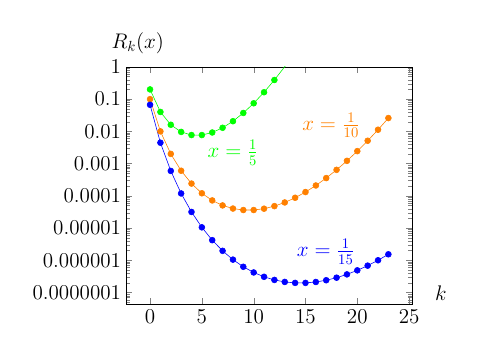
\begin{tikzpicture} [ scale=0.53, every mark/.append style={mark size=2pt} ]
\begin{axis}[
    ymode=log,
    log ticks with fixed point,
    ticklabel style = {font=\Large },
    ymax=1,
    x label style={font=\Large ,at={(axis description cs:1.1,0.1)}},
    y label style={font=\Large ,at={(axis description cs:0.15,1.1)},rotate=270},
    xlabel={$k$},
    ylabel={$R_k(x)$}
    % for log axes, y filter operates on LOGS.
    % and log(y * 1000) = log(y) + log(1000):
    % x filter/.code=\pgfmathparse{#1 + 6.90775527898214
]
\addplot  [
orange, mark=*
]  table {  % 1/10   % Print[Grid[   Table[{k, DecimalForm[N[Factorial[k]*(1/10)^(k + 1)]]}, {k, 0,    23}]]]
 0 0.10000000000000000000
 1 0.010000000000000000000
 2 0.0020000000000000000000
 3 0.00060000000000000000000
 4 0.00024000000000000000000
 5 0.00012000000000000000000
 6 0.000072000000000000000000
 7 0.000050400000000000000000
 8 0.000040320000000000000000
 9 0.000036288000000000000000
 10 0.000036288000000000000000
 11 0.000039916800000000000000
 12 0.000047900160000000000000
 13 0.000062270208000000000000
 14 0.000087178291200000000000
 15 0.00013076743680000000000
 16 0.00020922789888000000000
 17 0.00035568742809600000000
 18 0.00064023737057280000000
 19 0.0012164510040883200000
 20 0.0024329020081766400000
 21 0.0051090942171709440000
 22 0.011240007277776076800
 23 0.025852016738884976640
}
 node [pos=0.9 , above left, style={font=\Large}] {$x=\frac{1}{10}$};


\addplot  [
blue, mark=*
]  table {        % Print[Grid[   Table[{k, DecimalForm[N[Factorial[k]*(1/15)^(k + 1)]]}, {k, 0,    23}]]]
 0       0.0666667
1       0.00444444
2       0.000592593
3       0.000118519
4       0.0000316049
5       0.000010535
6       0.00000421399
7       0.00000196653
8       0.00000104882
9       0.000000629289
10      0.000000419526
11      0.000000307653
12      0.000000246122
13      0.000000213306
14      0.000000199085
15      0.000000199085
16      0.000000212358
17      0.000000240672
18      0.000000288807
19      0.000000365822
20      0.000000487762
21      0.000000682867
22      0.00000100154
23      0.00000153569
}
 node [pos=0.9 , above left, style={font=\Large}] {$x=\frac{1}{15}$};

\addplot  [
green, mark=*
]  table {        % Print[Grid[   Table[{k, DecimalForm[N[Factorial[k]*(1/5)^(k + 1)]]}, {k, 0,    23}]]]
 0       0.2
1       0.04
2       0.016
3       0.0096
4       0.00768
5       0.00768
6       0.009216
7       0.0129024
8       0.0206438
9       0.0371589
10      0.0743178
11      0.163499
12      0.392398
13      1.02024
14      2.85666
15      8.56997
16      27.4239
17      93.2413
18      335.669
19      1275.54
20      5102.17
21      21429.1
22      94288.0
23      433725.0
}
 node [pos=0.2 , below right, style={font=\Large}] {$x=\frac{1}{5}$};
\end{axis}
\end{tikzpicture}
\end{center}
\caption{Functional form of the absolute error $R_k(x)$ as a function of increasing $k$
for $x\in \{\frac{1}{5},\frac{1}{10},\frac{1}{15}\}$.}
  \label{2018-mm-ferror}
\end{marginfigure}
The functional form $k! x^k$ (times $x$) of the absolute error~(\ref{2011-m-ch-dseeanest})
suggests that, for $0<x<1$,
there is an ``optimal'' value $k \approx \frac{1}{x}$ with respect to convergence
of the partial sums $s(k)$ associated with Euler's asymtotic expansion of the solution~(\ref{2011-m-ch-dseess}):
up to this $k$-value the factor $x^k$ dominates the estimated absolute rest~(\ref{2011-m-ch-dseeest})
by suppressing it more than $k!$ grows.
However, this suppression of the absolute error as $k$ grows is eventually
-- that is, if $k > \frac{1}{x}$ -- compensated by the factorial function,
as depicted in Figure~\ref{2018-mm-ferror}: from $k \approx \frac{1}{x}$ the absolute error grows again,
so that the overall behavior of the absolute error $R_k(x)$  as a function of $k$ (at constant $x$)
is ``bathtub''-shaped; with a ``sink'' or minimum~\cite{rousseau-2004} at $k \approx \frac{1}{x}$.





One might interpret this behaviour as an example of what Boyd~\cite{Boyd99thedevil} refers to as
{\em Carrier's Rule}:
{\em ``Divergent series converge faster than convergent
series (because they don't have to converge); their
leading term is often a very good approximation.''}




% ListLogPlot[ Table[Factorial[k]*(1/10)^(k + 1), {k, 0, 23}]]
% Table[{k,N[Factorial[k]*(1/10)^(k + 1),20]}, {k, 0, 23}]


\begin{center}
{\color{olive}   \Huge
%\decofourright
 %\decofourright
%\decofourleft
%\aldine X \decoone c
 \floweroneright
% \aldineleft ]
% \decosix
%\leafleft
% \aldineright  w  \decothreeleft f \leafNE
% \aldinesmall Z \decothreeright h \leafright
% \decofourleft a \decotwo d \starredbullet
%\decofourright
% \floweroneleft
}
\end{center}
